\input{../tikz-header}
\begin{document}
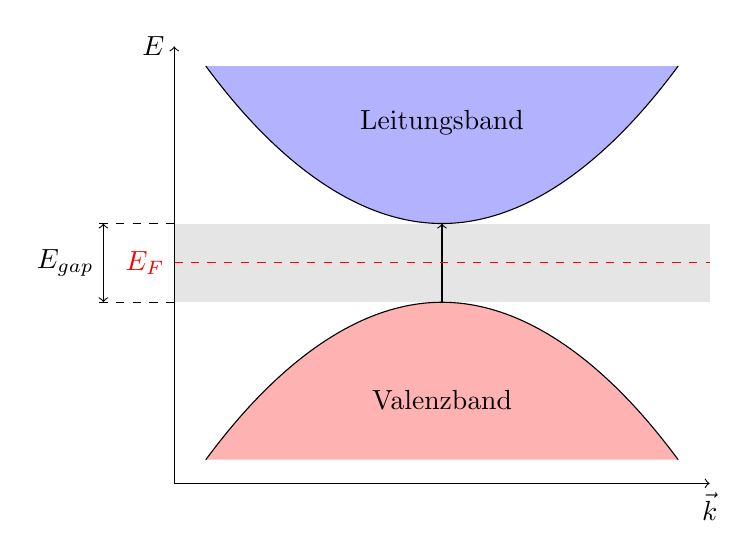
\begin{tikzpicture}
    \coordinate (LU) at (-3,0);
    \coordinate (CU) at (0,2);
    \coordinate (RU) at (3,0);
    \draw[fill=red, fill opacity=0.3] (RU) parabola bend (CU) (LU);
    \node[below, yshift=-1cm] at (CU) {Valenzband};

    \draw[->] (0,2) -- (0,3);

    \coordinate (LO) at (-3,5);
    \coordinate (CO) at (0,3);
    \coordinate (RO) at (3,5);
    \draw[fill=blue, fill opacity=0.3] (RO) parabola bend (CO) (LO);
    \node[above, yshift=1cm] at (CO) {Leitungsband};


    \draw[dashed] (-4.35,2) -- (-3.4,2);
    \draw[dashed] (-4.35,3) -- (-3.4,3);

    \fill[color=black, opacity=0.1] (-3.4,2) rectangle (3.4, 3);
    \draw[<->] (-4.3,2) -- node[left]{$E_{\text{gap}}$} (-4.3,3);

    \draw[color=red, dashed] (-3.4,2.5) node[left]{$E_F$} -- (3.4,2.5);
    \draw[->] (-3.4,-0.3) -- (-3.4,5.25) node[left]{$E$};

    \draw[->] (-3.4,-0.3) -- (3.4,-0.3) node[below]{$\lvert\vec{k}\rvert$};
\end{tikzpicture}
\end{document}